%% This is a sample file demonstrating the use of IJCAS.cls,
%% which is for the IJCAS (International Journal of Control, Automation, and Systems).
%%
%% 2004/03/08 by Karnes Kim
%% 2011/07/26 by CDSL, SNU
%%
%% Support sites: http://www.ijcas.com
%%
%% This code is offered as-is - no warranty - user assumes all risk.
%% Free to use, distribute and modify.
%%

%% The IJCAS class supports two column page basically. 
%%So, you need not use two column option or command.
\documentclass{IJCAS}

%% include the useful LaTeX packages:
\usepackage{url}
\usepackage{array,tabularx}
\usepackage{multicol} 

%%%% Editorial Information
%% Authors do not have to modify this section.
\journalvolumn{VV}
\journalnumber{X}
\journalyear{YYYY}
\setarticlestartpagenumber{1}
%%%% End of Editorial Information

%The environment for theorem, lemma, remark, corollary, proposition, and definition are already defined.


%The following command is needed for line break of long equations.
\allowdisplaybreaks


\begin{document}
% the \title command
\title{Manuscript Template for the International Journal of Control, Automation, and Systems: ICROS \& KIEE}

% the \author command
% the \orcid{orcid number}
\author{Gil-Dong Hong*, Adam Smith, and Ikuro Mizumoto}

% the abstract environment
\begin{abstract}
This article describes the preparation procedure for publication in the International Journal of Control, Automation, and Systems (IJCAS), and this template applies both for initial submission and the final camera-ready manuscript of the paper. When authors submit their work for review, it is necessary to follow these instructions. The abstract should not exceed 300 words for regular papers or 75 words for technical notes and correspondence without equations, references, and footnotes.
\end{abstract}

\begin{keywords}
At least four keywords or phrases in alphabetical order, separated by commas.
\end{keywords}

\maketitle

\makeAuthorInformation{
Manuscript received January 10, 2026; revised March 10, 2026; accepted May 10, 2026. Recommended by Associate Editor Soon-Shin Lee under the direction of Editor Milton John.\\

Gil-Dong Hong is with the School of Electrical and Computer Engineering, Best University, 635-4 Yeoksam-dong, Gangnam-gu, Seoul 12345, Korea (e-mail: journal@ijcas.com). Adam Smith and Ikura Mizumoto are with the School of Mechanical Engineering, World University, 1050 Jackson St., Albany, CA 94000, USA (e-mails: \{smith, newton\}@icros.org).

* Corresponding author.
}

\runningtitle{2026}{Gil-Dong Hong, Adam Smith, and Ikuro Mizumoto}{Manuscript Template for the International Journal of Control, Automation, and Systems: ICROS {\&} KIEE}{xxx}{xxxx}{x}




\section{INTRODUCTION}

This document is a template for LATEX users. If you are reading a printed version of this document, please download an electronic file, IJCAS manuscript template.zip, from \urlstyle{rm}\url{https://ijcas.com}. You can use this template to prepare your manuscript. If you prefer to use MS Word template file, please download the IJCAS' Microsoft Word style and sample files from the same website. We recommend you to use LATEX for fast typesetting and publication schedule because the published file will be based on LATEX. But, we also accept Microsoft \textit{Word} files for the authors' convenience.

It is necessary to adhere to these instructions when a manuscript is submitted for review. It is highly recommended to submit the manuscript in a \textit{two-column format using template.} \textit{The authors must strictly follow these instructions} to maintain the high standard of the journal. 

A manuscript is divided into three parts: The first part includes the title, authors' names, abstract, and keywords. The second part is the paper's main body including the conclusion section, and the third part is the authors' profile section at the end.



\section{PAPER SIZE AND FORMAT}



The paper size should be A4, and the following margins should be set:\\

\begin{tabular}{p{1.1in}p{1.1in}}  
Left margin                & 20 mm \\  
\end{tabular}\\[-1pc]

\vskip -0.5pc
\begin{tabular}{p{1.1in}p{1.1in}} 
Right margin                       & 20 mm \\ 
Top margin             & 30 mm \\  
Bottom margin & 30 mm \\  
Heading & 10 mm 
\end{tabular}\\

\noindent
Also, using the above margins, the article can be printed on U.S. Letter size papers.\\

\noindent
The paper should be within the allowed page length.
\begin{itemize}\setlength{\itemindent}{0.5pc}
\item[1)] Regular papers: Up to 10 pages
\item[2)] Technical notes and correspondence: Up to 5 pages
\end{itemize}

\noindent
The page length is measured in the two-column format of this template. An over-length paper can be considered, but a justification is necessary when the initial submission is made. An over-length charge will be applied for publication if accepted.



\section{FONTS AND STYLE}

\subsection{First part}

The first part includes the paper title, authors' names, abstract, and keywords. All fonts must be in Times New Roman, and the font sizes of the title, authors' names, abstract, and keywords are 14 pt (bold), 10 pt (bold), 10 pt, and 10 pt, respectively.



\subsection{Paper body}

The second part of the manuscript's main body must be edited in double-column format, with each column 80 mm in width and separated by 8 mm. The top-level heading, usually called section and numbered in Roman numerals, shall appear centered on the column with Times New Roman capital bold 10 pt. The numbered level-two heading must be shown in Times New Roman 10 pt font.\\[0.75pc]
%
The main text uses Times New Roman 10 pt with single line spacing. A new paragraph starts with a 3.5 mm indentation. However, if an empty line exists before a new paragraph, it can start without an indentation. \\[0.75pc]
%
If you hit a return key after putting an equation number, the computer assumes that you want to go to a new paragraph, which is not the case. Therefore, you must remove the indentation automatically made after hitting the return key.



\subsection{Subsection}

The numbering of the subsection should take the above form.



\section{FIGURE / TABLE / EQUATION}

\subsection{Figure}

Clear original figures should be used. The authors should submit the original graphic files separately along with the main article file (for the camera-ready version after acceptance). The preferred formats for graphics are Tagged Image File (.tif), Encapsulated Postscript (.eps), and JPG (.jpg) format. High-contrast line figures should be prepared with 600 dpi resolution, and color/gray figures should be prepared with more than 300 dpi resolution. The color figures should be distinguished even if the figures are printed with black and white printers. 

\begin{figure}[!t]
\begin{center}
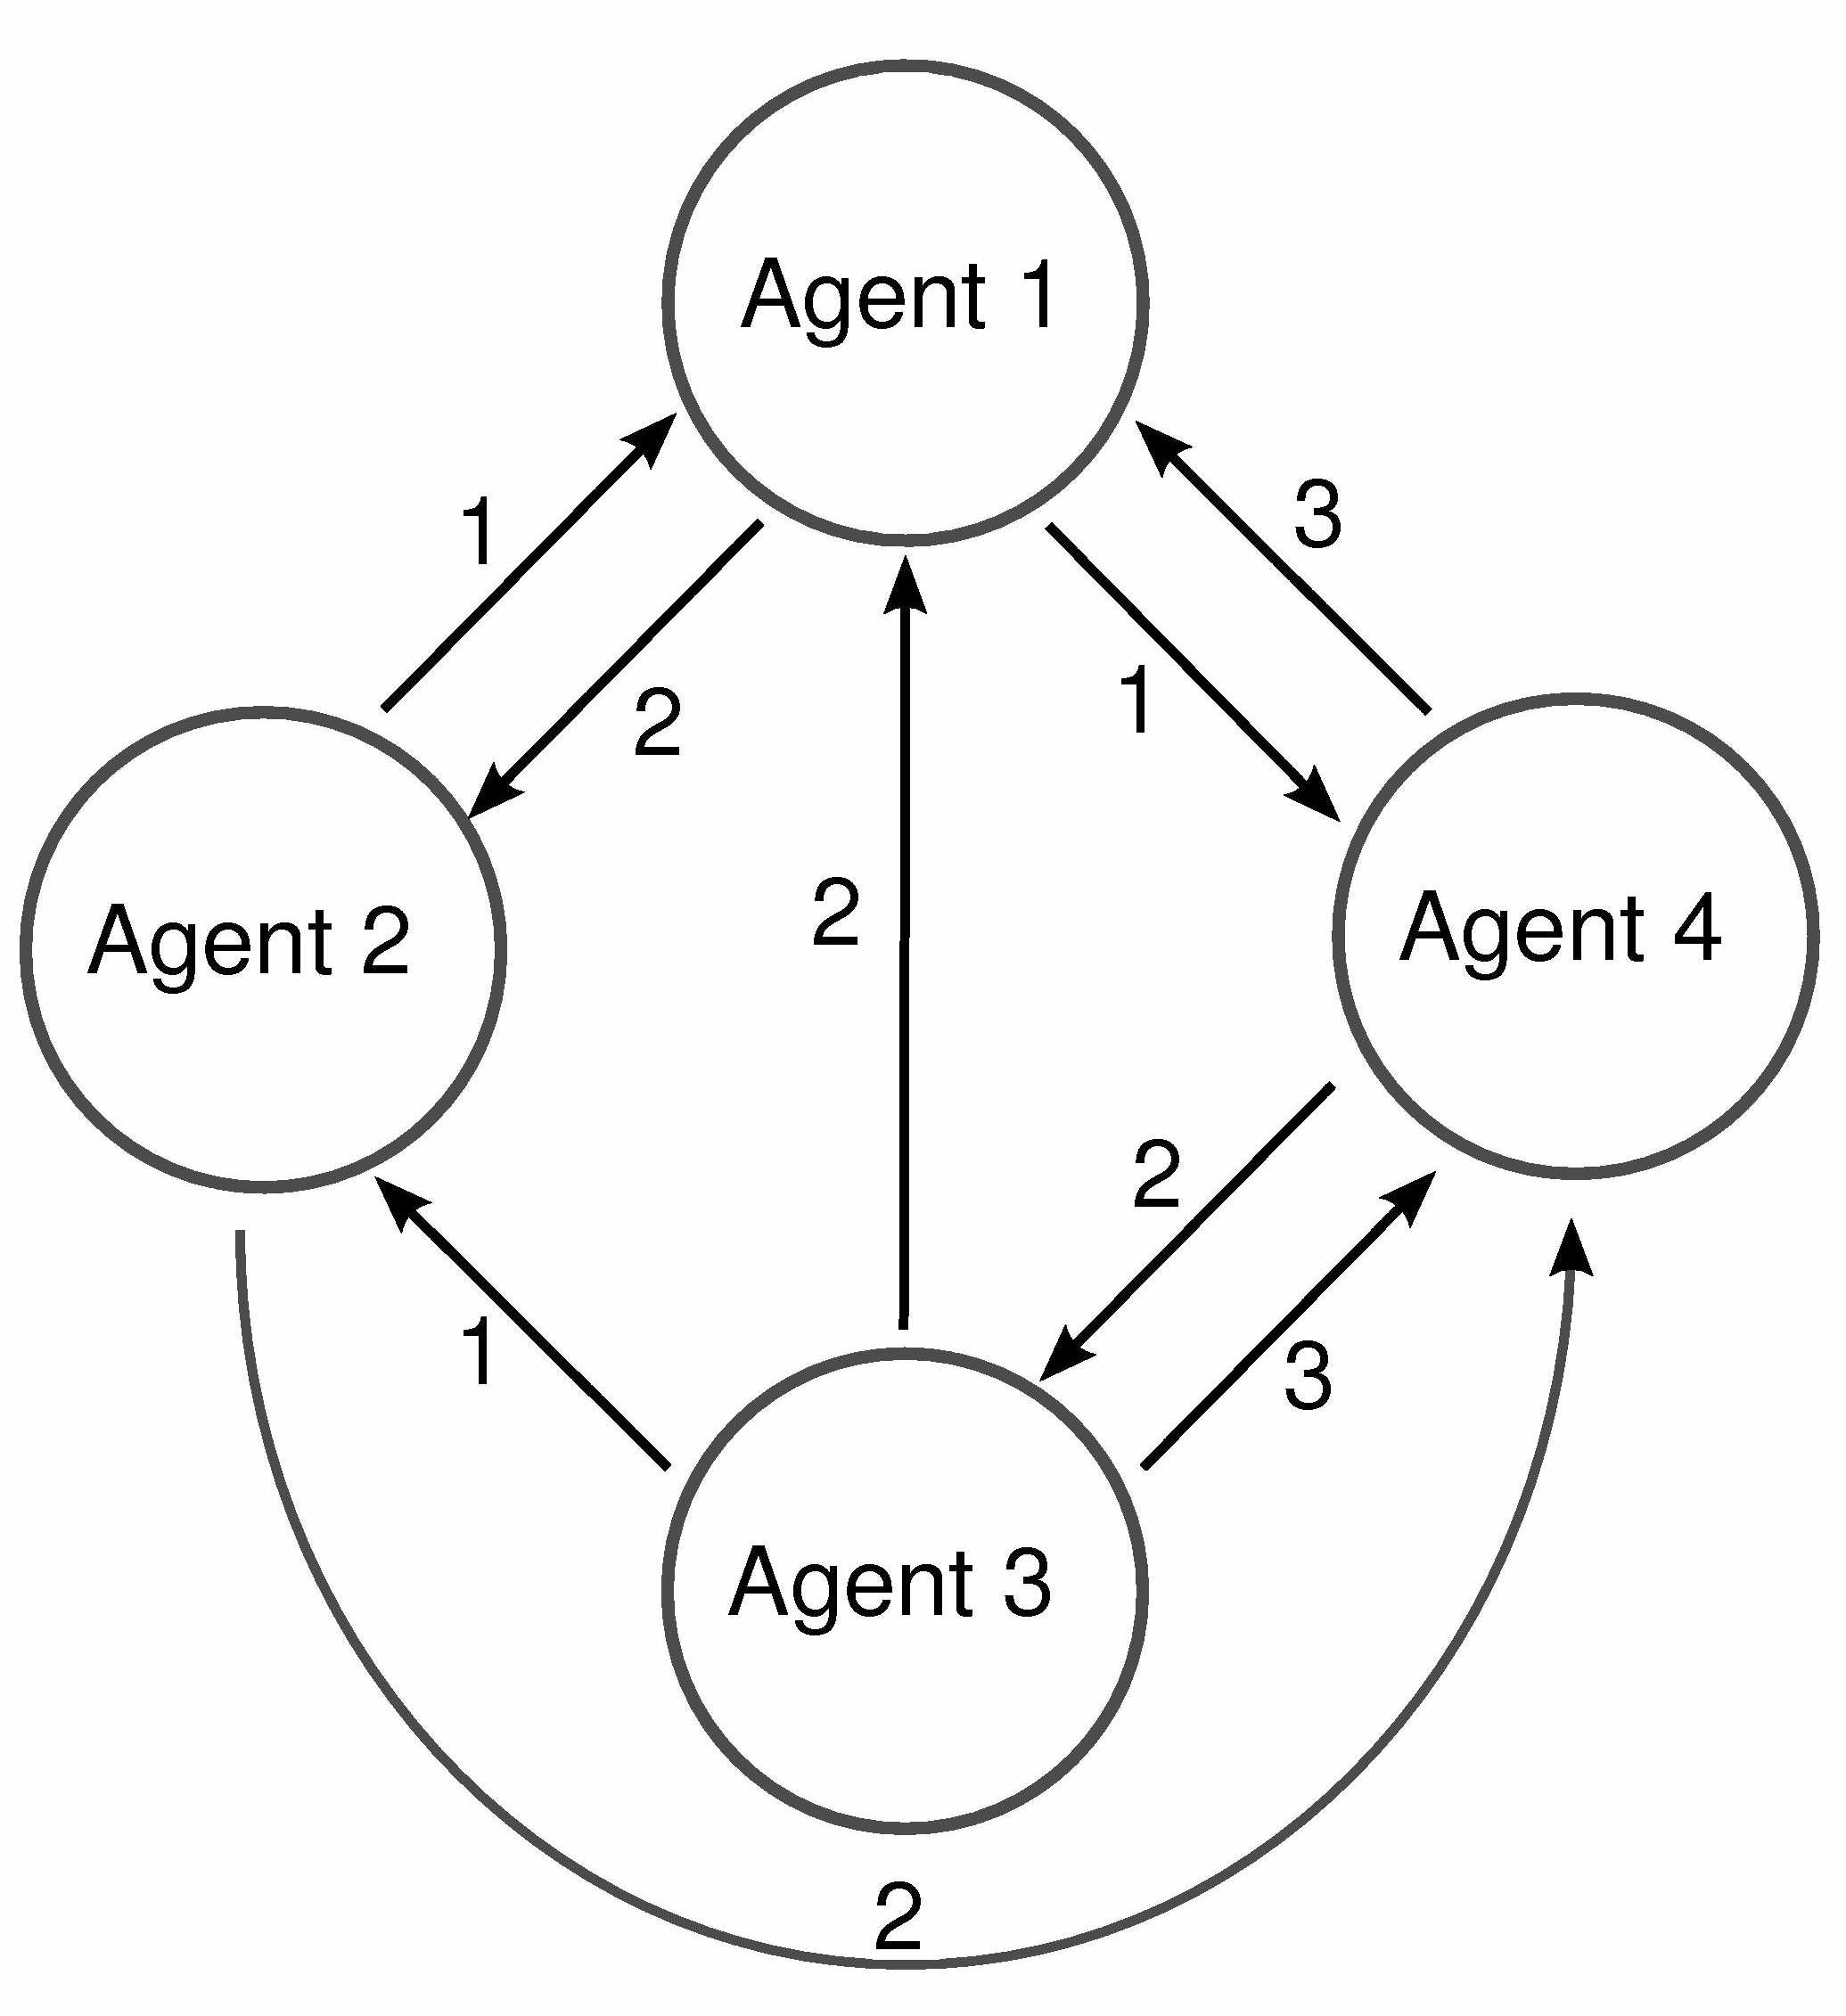
\includegraphics[width=4.75cm]{fig1} 
\vskip -0.5pc
\caption{The caption must be shown after the figure.}\label{fig:1}
\end{center}
\vskip -1.5pc
\end{figure}


\begin{table}[!b] 
\vskip -0.75pc
\setlength{\extrarowheight}{0.5ex}
\setlength{\tabcolsep}{1pt}
\caption{The caption must be shown before the table.}\label{tab:1}
\begin{center}
\vskip -1.25pc
{\footnotesize
\begin{tabu}to\linewidth{|X[c]|X[c]|X[c]|X[c]|} 
\hline 
  & A & B & C \\ \hline 
(1) & 150\% & 16.3\% & 18.2\% \\ \hline 
(2) & 31.1\% & 33.8\% & 29.8\% \\ \hline 
(3) & 13.3\% & 12.1\% & 11.1\% \\ \hline 
\end{tabu}
}
\end{center}
\vskip -0.25pc
\end{table}

\subsection{Table}
\newpage





\subsection{Equation}

The equations should be numbered serially throughout the paper. The equation number should be located to the far right of the line in parenthesis. Equations are shown left aligned on the column.

\begin{theorem}
Equations are made as follows:
\begin{align} 
&\label{eq:1} 
\dot{x}=Ax+Bu, \\
&\label{eq:2} 
y=Cx+Du. 
\end{align} 
You must remove all the automatically-made indentations made after hitting the return key. 
\end{theorem}
\begin{proof}
Each equation should be separated by a comma. Assuming that the Equation Editor is used, the settings for individual font sizes are

Main equation: 10 pt (Times New Roman),

Subscript/superscript: 7 pt (Times New Roman),

Sub-subscript: 6 pt (Times New Roman),

Symbol: 150\%,

Sub-symbol: 100\%. 

The equation number should be set with a right tap as shown in \eqref{eq:1}-\eqref{eq:2}. This is the end of the proof.
\end{proof}



\begin{remark}
The journal office knows how to convert all equations into font 10 pt at once. Please inquire about this before preparing the final manuscript. This will be handy for you.
\end{remark}



\subsection{Equation/figure/table citation}

Equations \eqref{eq:1}-\eqref{eq:2} stand for the system dynamics. Fig. \ref{fig:1} is the first figure. Table \ref{tab:1} is cited as such. In the paper, all authors are required to use the SI unit.


\subsection{References}

References should appear in a separate bibliography at the end of the paper, with items referred to by numerals in square brackets \cite{1,3,4,5}. Times New Roman 10 pt is used for references \cite{2}. References should be complete in the IJCAS style shown in the Reference section of this article. An article should include vol., no., pages, and year.



\subsection{Author information}

Brief biographies and either clear glossy photographs (25 mm $\times$ 30 mm) of the authors or TIF files of the figures should be submitted after the paper is accepted.



\section{CONCLUSION}

The authors should prepare their article for initial and final submission following the ``Information for Authors? available at \href{http://ijcas.com}{http://ijcas.com} and this file. If accepted, the authors will be required to provide the text of the final version of their manuscript to the journal office. 



\appendix

The author(s) can insert an appendix with a meaningful title here.



\section*{DECLARATIONS}

\subsection*{Conflict of Interest}
Always applicable and includes interests of a financial or personal nature. For example, ``The authors declare that there is no competing financial interest or personal relationship that could have appeared to influence the work reported in this paper.''

\subsection*{Authors' Contributions}
If there is one more author, please ensure that all authors' contributions are individually mentioned with their full names.

\subsection*{Funding }
It should be provided in the Declarations, separate from the Acknowledgements. If any of these declarations listed are not relevant to the content of your submission, please state that this declaration is ``Not Applicable''.

\subsection*{Data Availability}
An article’s data availability statement lets a reader know where and how to access data that support the results and analysis. It may include links to publicly accessible datasets that were analyzed or generated during the study, descriptions of what data are available and/or information on how to access data that is not publicly available. 



\begin{reference}
\bibitem{1} \doi{R. C. Baker and B. Charlie, ``Nonlinear unstable systems,'' \textit{International Journal of Control}, vol. 23, no. 4, pp. 123-145, 1989.}{10.1007s/s12555-xxx-xxxx-x}

\bibitem{2} G.-D. Hong, ``Linear controllable systems,'' \textit{Nature}, vol. 135, no. 5, pp. 18-27, 1990. 

\bibitem{3} K.-S. Hong and C. S. Kim, ``Linear stable systems,'' \textit{IEEE Transactions on Automatic Control}, vol. 33, no. 3, pp. 1234-1245, 1993. 

\bibitem{4} Z. Shiler, S. Filter, and S. Dubowski, ``Time optimal paths and acceleration lines of robotic manipulators,'' \textit{Proc. of the 26th Conference on Decision and Control}, pp. 98-99, 1987.

\bibitem{5}  M. Young, \textit{The Technical Writer's Handbook}, Mill Valley, Seoul, 1989.

\bibitem{6}  Y. Feng, H. Wang, H. Lu, C. Chang, L. Luo, and F. Yang, ``A novel faster all-pair shortest path algorithm based on the matrix multiplication for GPUs,'' \textit{arXiv preprint} arXiv:2208.04514, 2022.

\bibitem{7} ``Reinforcement learning,'' Wikipedia, [Online]. Available: \href{https://en.wikipedia.org/wiki/Reinforcement_learning}{https://en.wikipedia.org/wiki/Reinforcement\_learning}. [Accessed: March 24, 2025].
\end{reference}


\biography{author.jpg}{Gil-Dong Hong}{(Times New Roman 9 pt, Bold) received his B.S. degree in Electrical Engineering from Best University in 2003. His research interests include nonlinear control, adaptive control, and system identification.}

\clearafterbiography
\relax 

\end{document}

